\chapter{Testy}

\section{Debugowanie aplikacji i dostęp do informacji o jej działaniu}
Do wykonywania debugowania aplikacji w celu znalezienia błędów użyto wtyczki do programu \textit{Visual Studio Code} oraz wbudowanego w przeglądarkę internetową \textit{Google Chrome}, debuggera dostępnego z poziomu panelu narzędzi deweloperskich (zakładka \textit{Sources}) widoczna na rysunku \ref{Rys:sources} . W tym miejscu możliwe jest podejrzenie i debugowanie skryptów aplikacji. Programista ma również możliwość śledzenia wybranych wyrażeń (pole \textit{Watch expressions}), przeglądania stosu aplikacji (pole \textit{Call Stack}), ustawiania tzw. \textit{breakpointów} w momencie debugowania, przechodzenia kodu krok po kroku i wiele, wiele innych.

\begin{figure}[h]
	\centering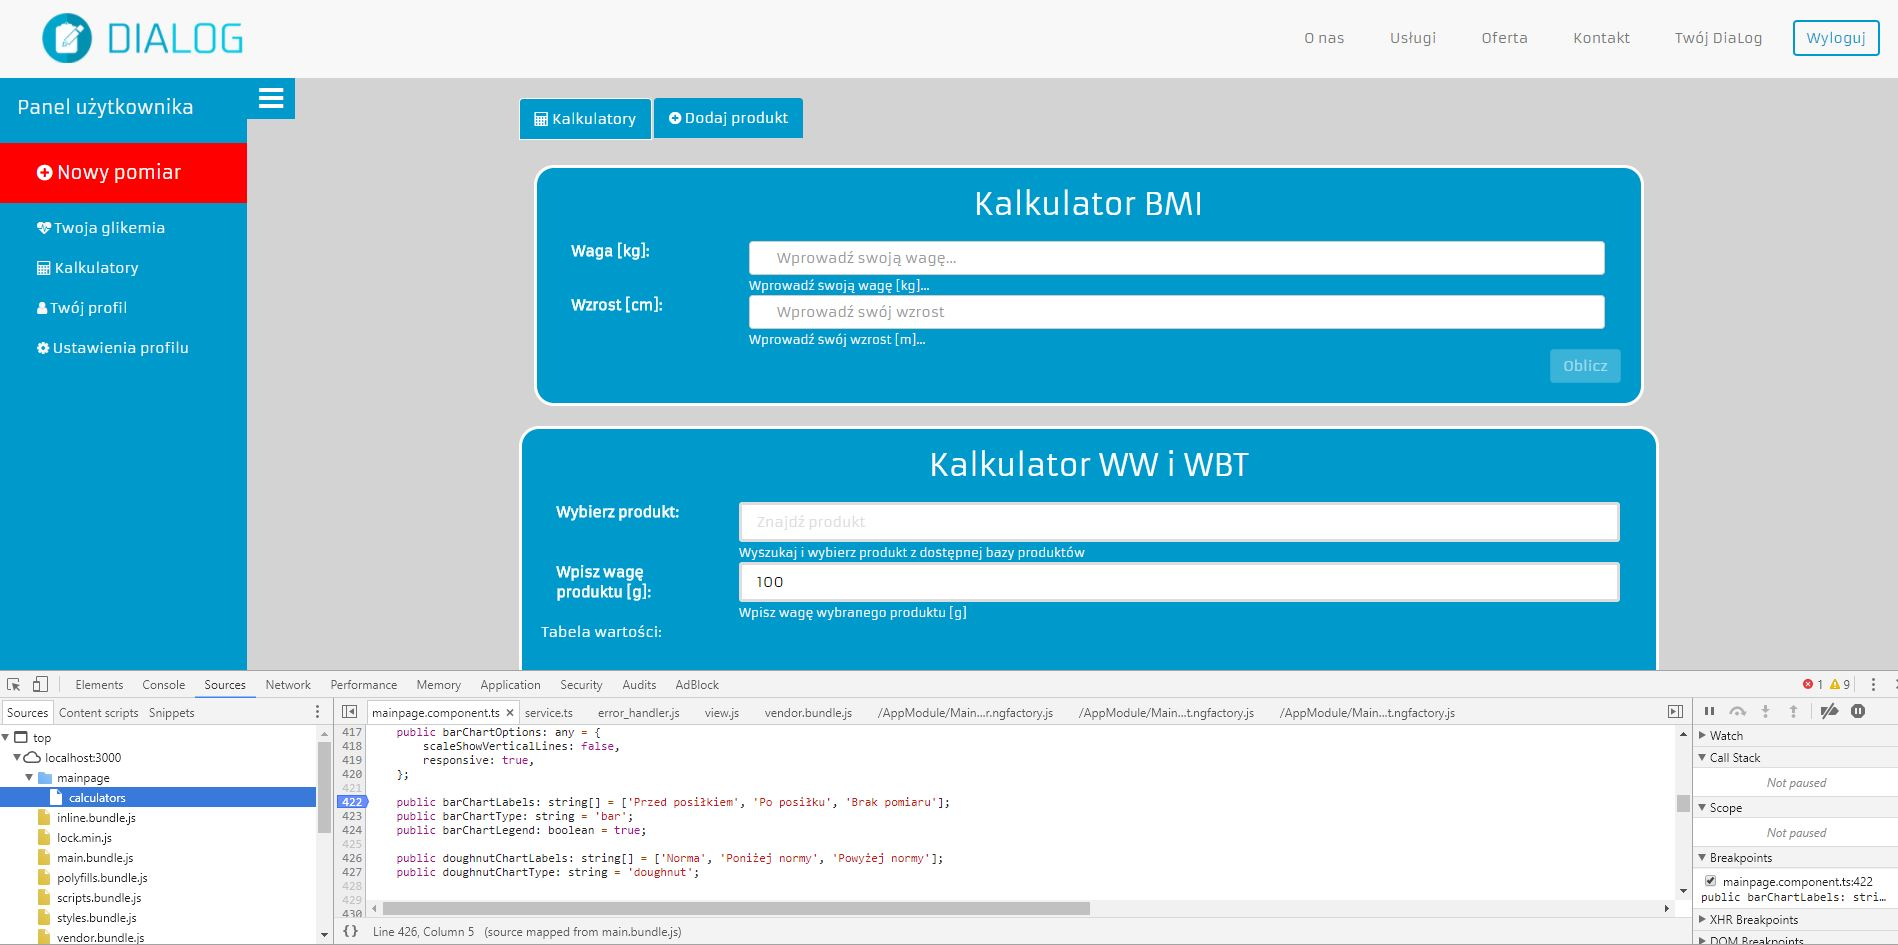
\includegraphics[scale=0.3]{images/sources.jpg}
	\caption{Opcje debugowania i podglądu kodu dostępne z poziomu zakładki \textit{Sources} narzędzi deweloperskich przeglądarki \textit{Google Chrome}}
	\label{Rys:sources}
\end{figure}


Do podglądu poprawności wysyłanych żądań za pomocą metod HTTP użyto narzędzi dostępnych z poziomu zakładki \textit{Network}. Oferuje ona podgląd adresów URL (\textit{Uniform Resource Locator}) generowanych do pobrania danych w formacie JSON oraz treści tablicy obiektu zawierającego te dane (rys. \ref{Rys:network}).
 
 \begin{figure}[h]
 	\centering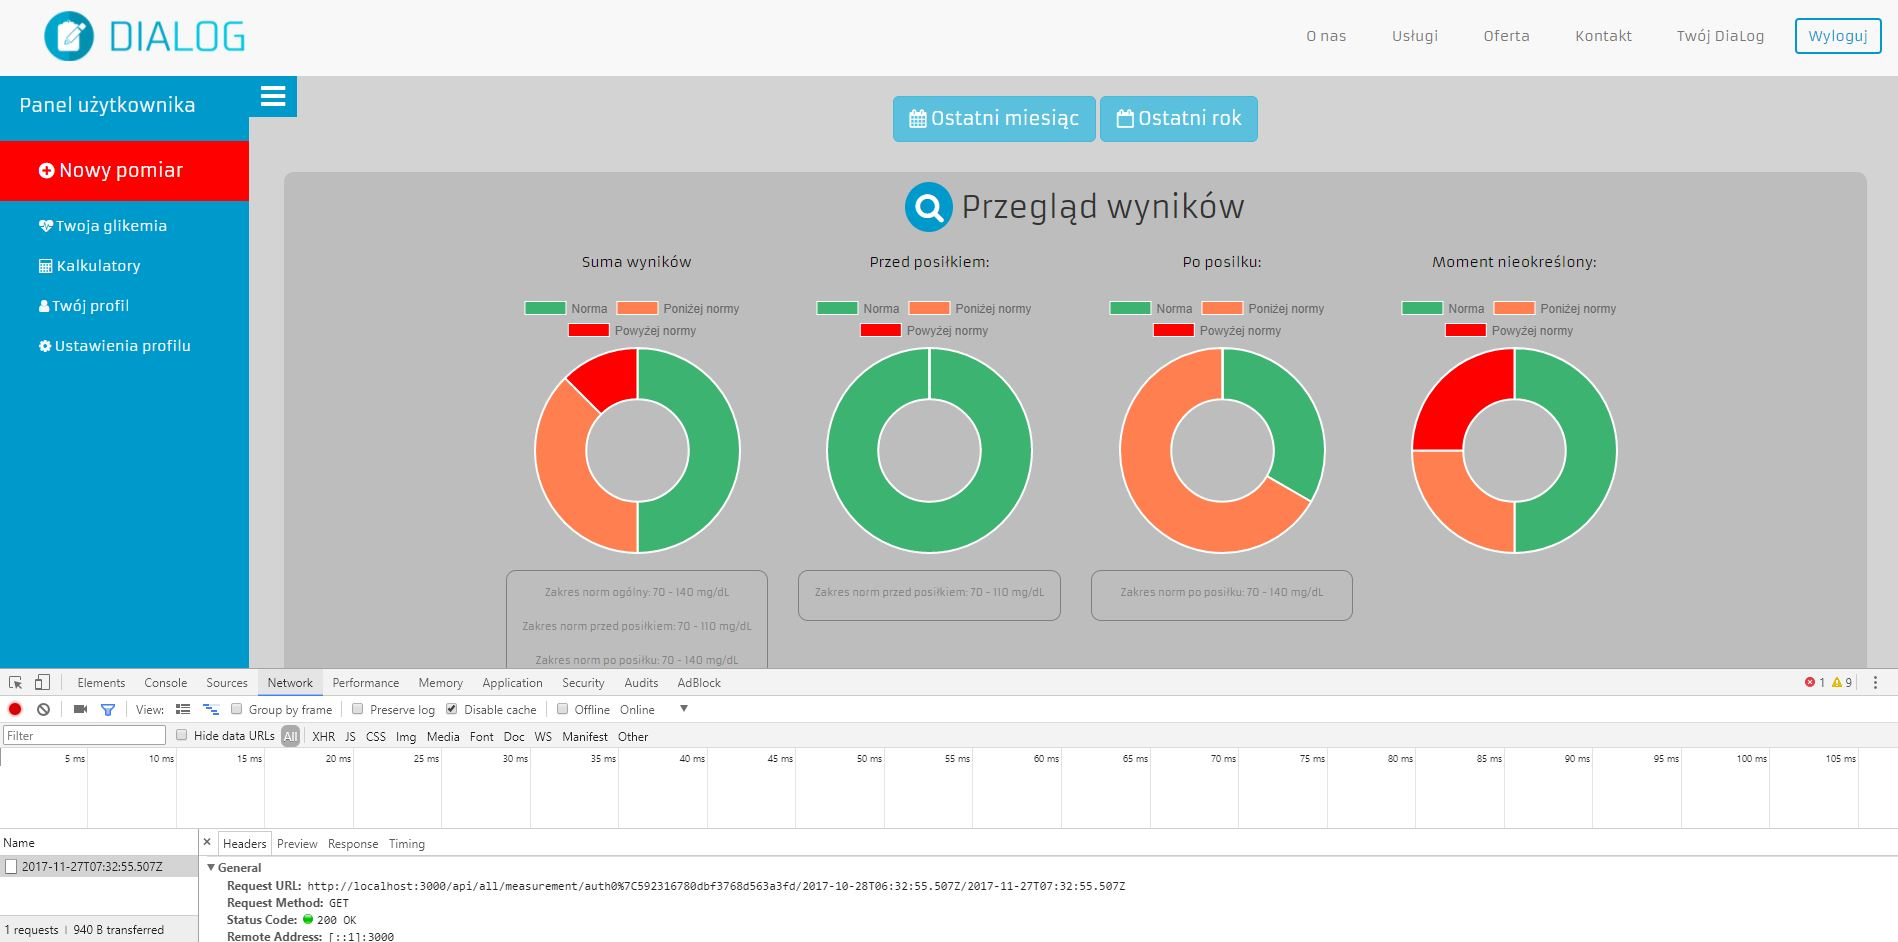
\includegraphics[scale=0.3]{images/network.jpg}
 	\caption{Opcje podglądu przesyłanych żądań dostępne z poziomu zakładki \textit{Network} narzędzi deweloperskich przeglądarki \textit{Google Chrome}}
 	\label{Rys:network}
 \end{figure}

\newpage
  
W celu identyfikacji rodzaju błędu posłużono się oknem konsoli dostępnym z poziomu zakładki \textit{Console}. Oferuje ona dokładny opis zaistniałego błędu wraz ze ścieżką lokalizacji do pliku z~ błędnym fragmentem kodu, a nawet numeru linijki, w której dany błąd wystąpił. W przypadku użycia metod HTTP (\textit{Hypertext Transfer Protocol}) wyświetlany jest odpowiedni numer błędu zgodnie ze specyfiacją kodów błędów HTTP. W oknie konsoli możliwy jest również podgląd wartości przechowywanych przez zmienne w projekcie oraz dostęp do treści ostrzeżeń w trakcie działania aplikacji (rys. \ref{Rys:console}).
 

 \begin{figure}[h]
	\centering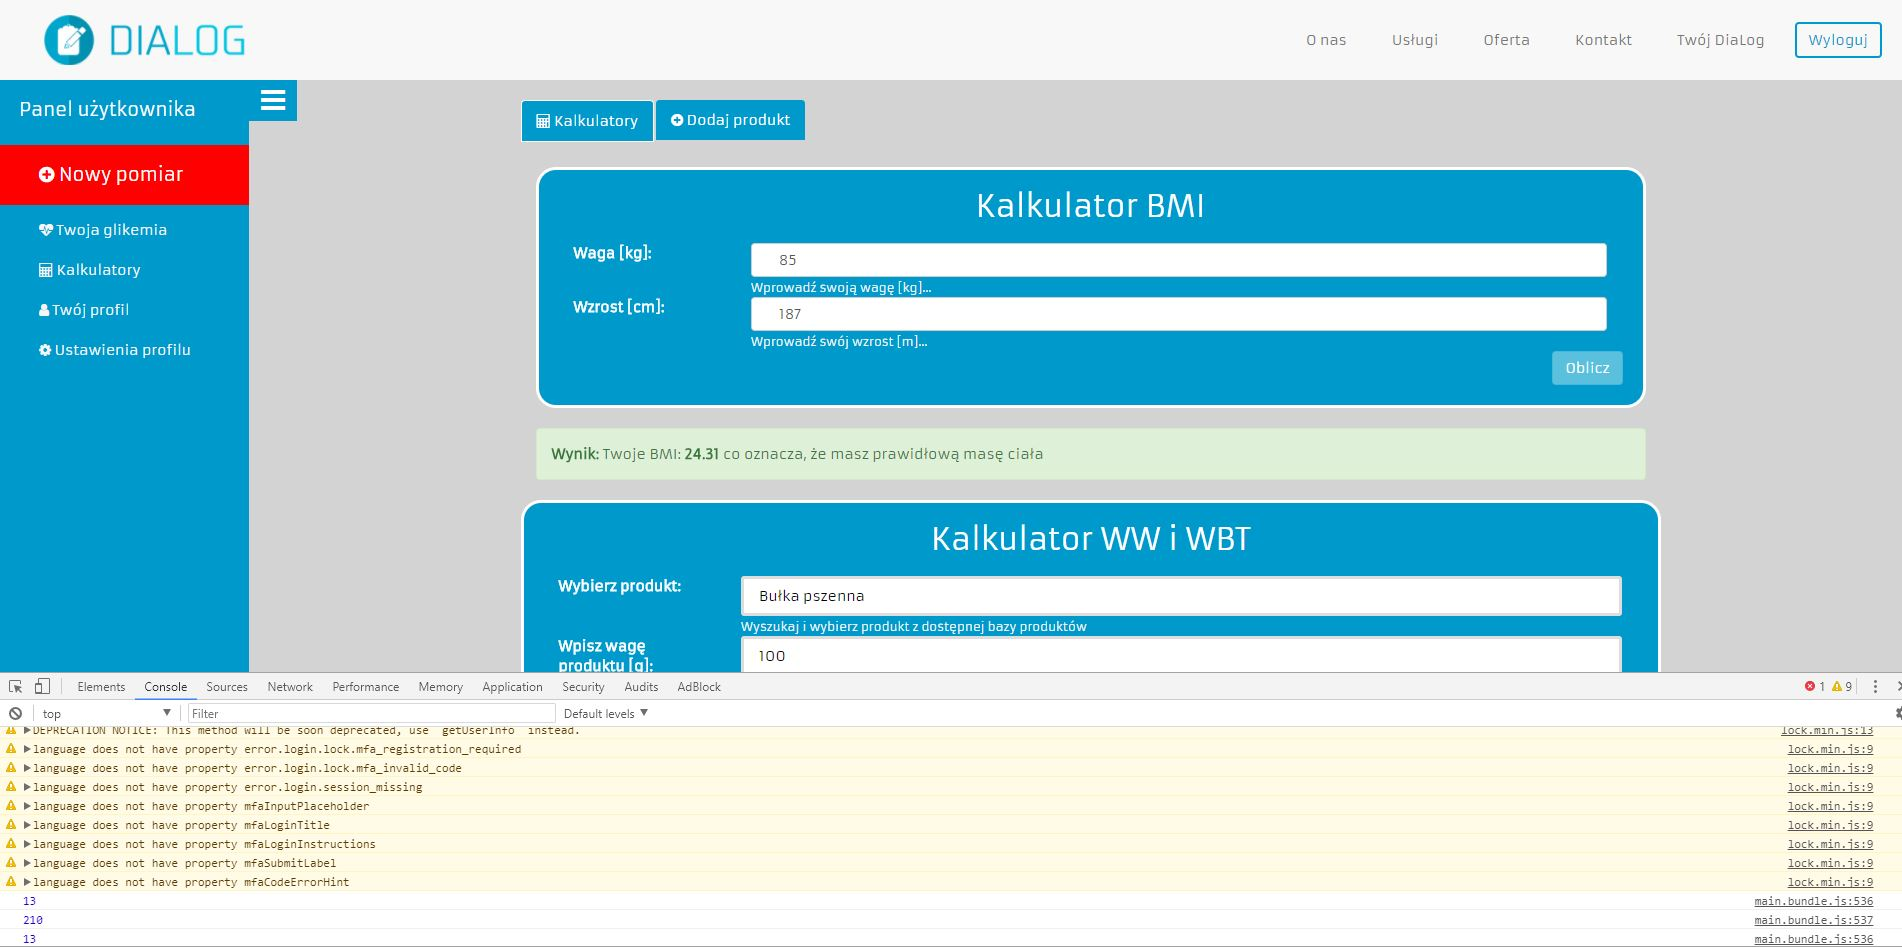
\includegraphics[scale=0.3]{images/console.jpg}
	\caption{Opcje podglądu błędów, ostrzeżeń i wartości zmiennych dostępne z poziomu zakładki \textit{Console} narzędzi deweloperskich przeglądarki \textit{Google Chrome}}
	\label{Rys:console}
 \end{figure}

\section{Testy funkcjonalne aplikacji}

Aplikację skonstruowano pod kątem UX (\textit{User Experience}), a kod napisano w~ oparciu o podstawowe zasady budowania struktury projektu tworzonego z wykorzystaniem frameworku \textit{Angular 2} \cite{Ans}. Dołożono wszelkich starań, aby ilość danych umieszczanych w~ ramach jednego widoku nie była zbyt duża, ponieważ w~ przypadku \textit{Angulara 2} znacząco obniża to wydajność aplikacji. 

W ramach testów funkcjonalnych aplikacji przeprowadzono podstawowe czynności mające na celu zapewnienie stabilności jej działania. Zostały one wykonane zgodnie z założeniami funkcjonalnymi, jakie powinien spełniać program. Pierwszym krokiem było sprawdzenie poprawności wysyłanych do serwera żądań (\textit{Requests}) w celu pobrania danych (\textit{Response Data}). Posłużono się oprogramowaniem \textit{Postman}. 

Każda z metod HTTP (\textit{Hypertext Transfer Protocol}) służących do komunikacji z serwerem w celu pobrania lub wysłania danych została sprawdzona poprzez wprowadzenie najpierw błędnych, a następnie poprawnych parametrów w nagłówku, bądź w adresie URL (\textit{Uniform Resource Locator}) metody. Przykładowe wyniki testu przedstawiono na rysunkach \ref{Rys:postman_fail} oraz \ref{Rys:postman_good}.

\begin{figure}[h]
	\centering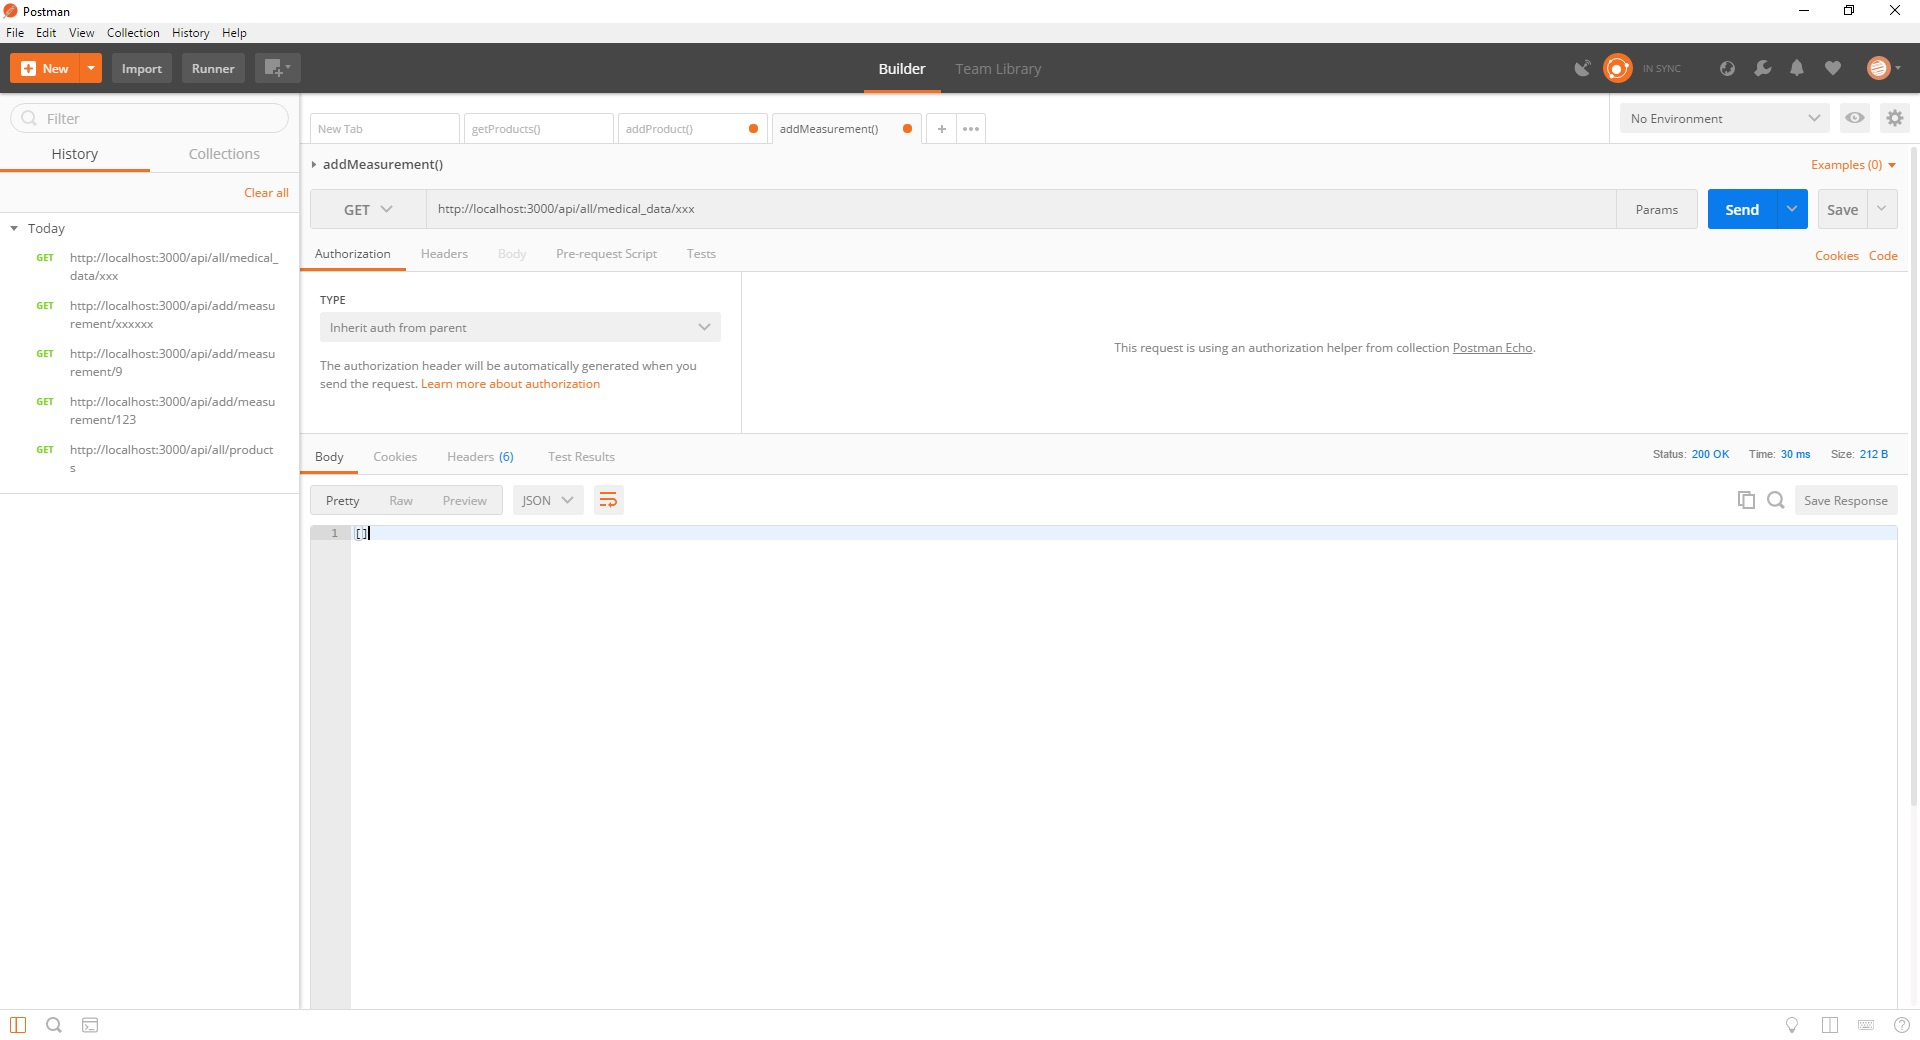
\includegraphics[scale=0.3]{images/postman.JPG}
	\caption{Próba pobrania danych medycznych za pomocą oprogramowania \textit{Postman} użytkownika o błędnym identyfikatorze}
	\label{Rys:postman_fail}
\end{figure}

W przypadku wprowadzenia błędnego identyfikatora użytkownika w adresie URL metody GET służącej do pobrania jego danych medycznych uzyskano odpowiedź z serwera z pustą tablicą danych. 

Przy próbie wprowadzenia poprawnego identyfikatora w adresie URL tej samej metody serwer zwrócił żądane dane medyczne użytkownika.

\newpage

\begin{figure}[h]
	\centering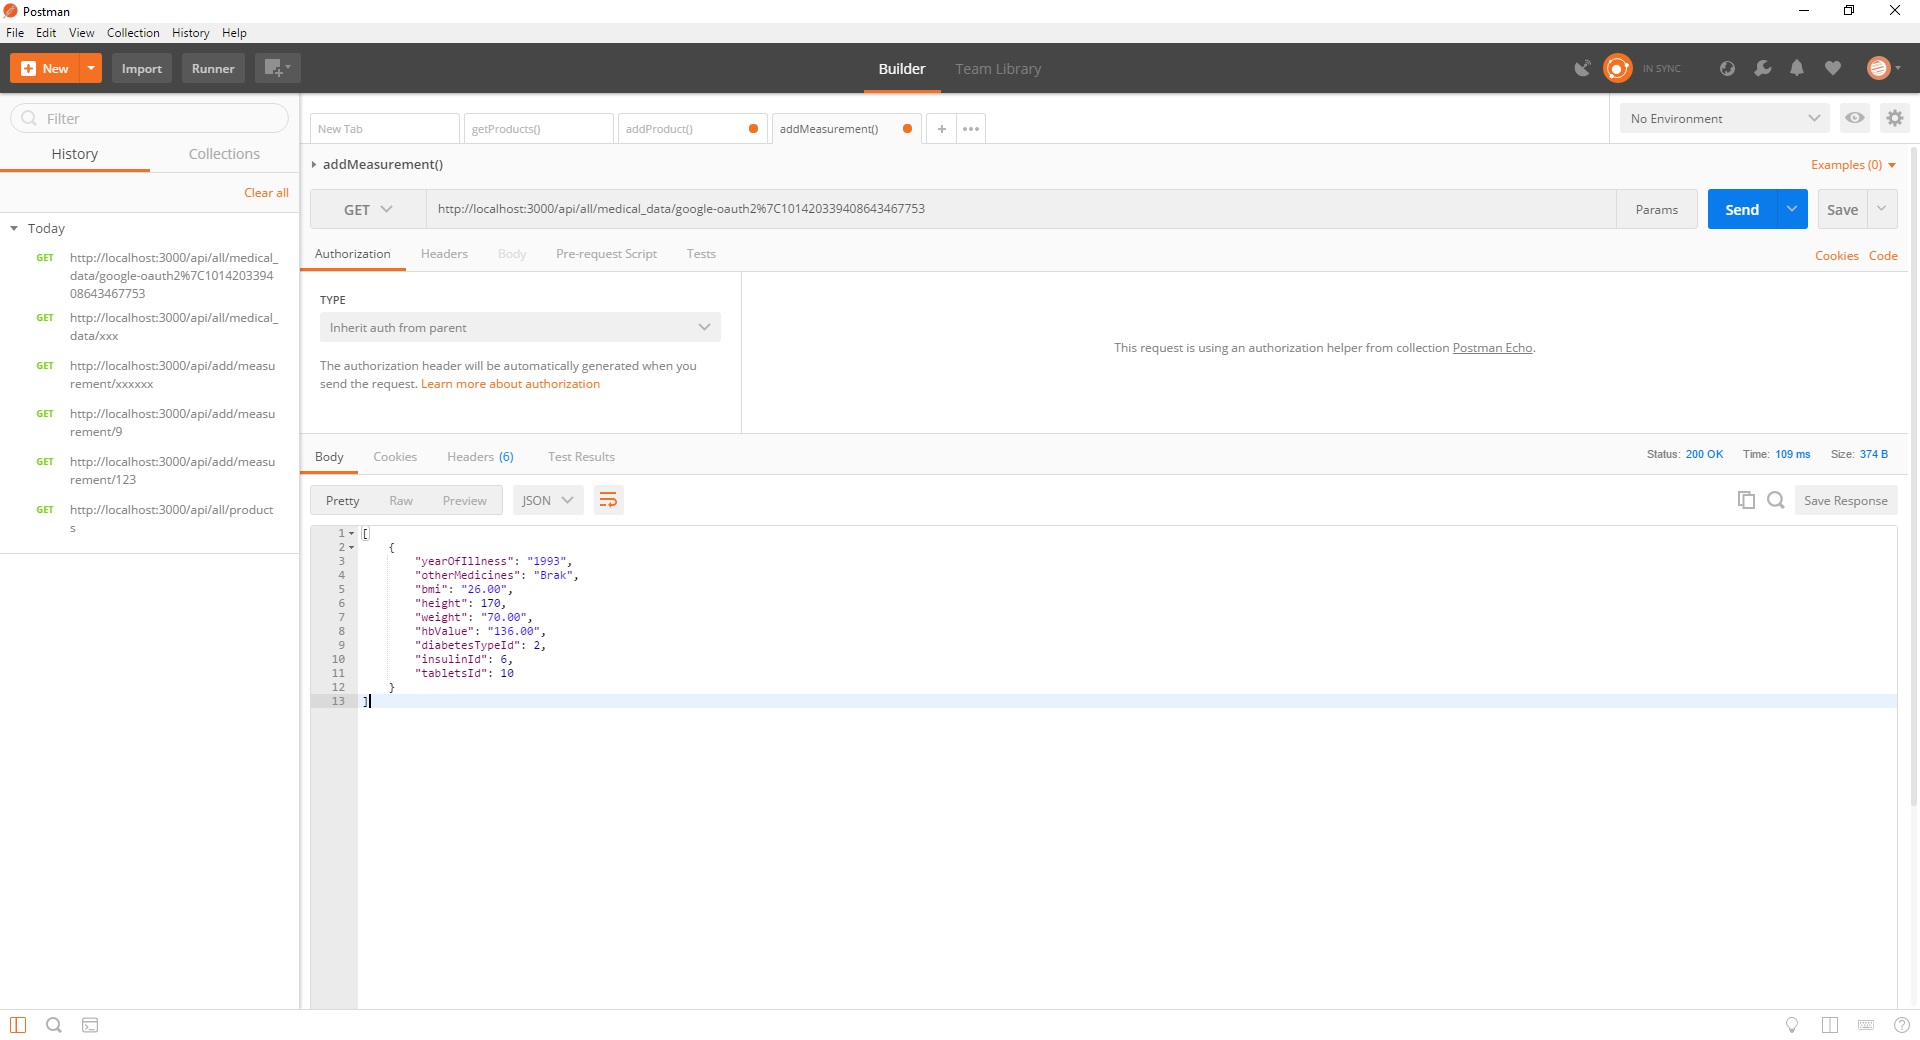
\includegraphics[scale=0.3]{images/postman2.JPG}
	\caption{Próba pobrania danych medycznych za pomocą oprogramowania \textit{Postman} użytkownika o poprawnym identyfikatorze}
	\label{Rys:postman_good}
\end{figure}

Kolejną czynnością było sprawdzenie poprawności walidacji danych w formularzach aplikacji. Reguły walidacji odpowiednich pól określone zostały przy użyciu wyrażeń regularnych. Zastosowano odpowiedni przycisk powiązany bezpośrednio z formularzem, służący do wysyłania żądania z uzupełnionymi danymi. Zablokowano go do momentu kiedy użytkownik nie wprowadzi poprawnych danych. Takie podejście zabezpiecza program przed błędami związanymi z niezgodnością typów w bazie danych. Pozwala również uniknąć zapisywania informacji (takich jak kod pocztowy) w niewłaściwym formacie (rys. \ref{Rys:form}) \cite{Ang}. 
  
\begin{figure}[h]
	\centering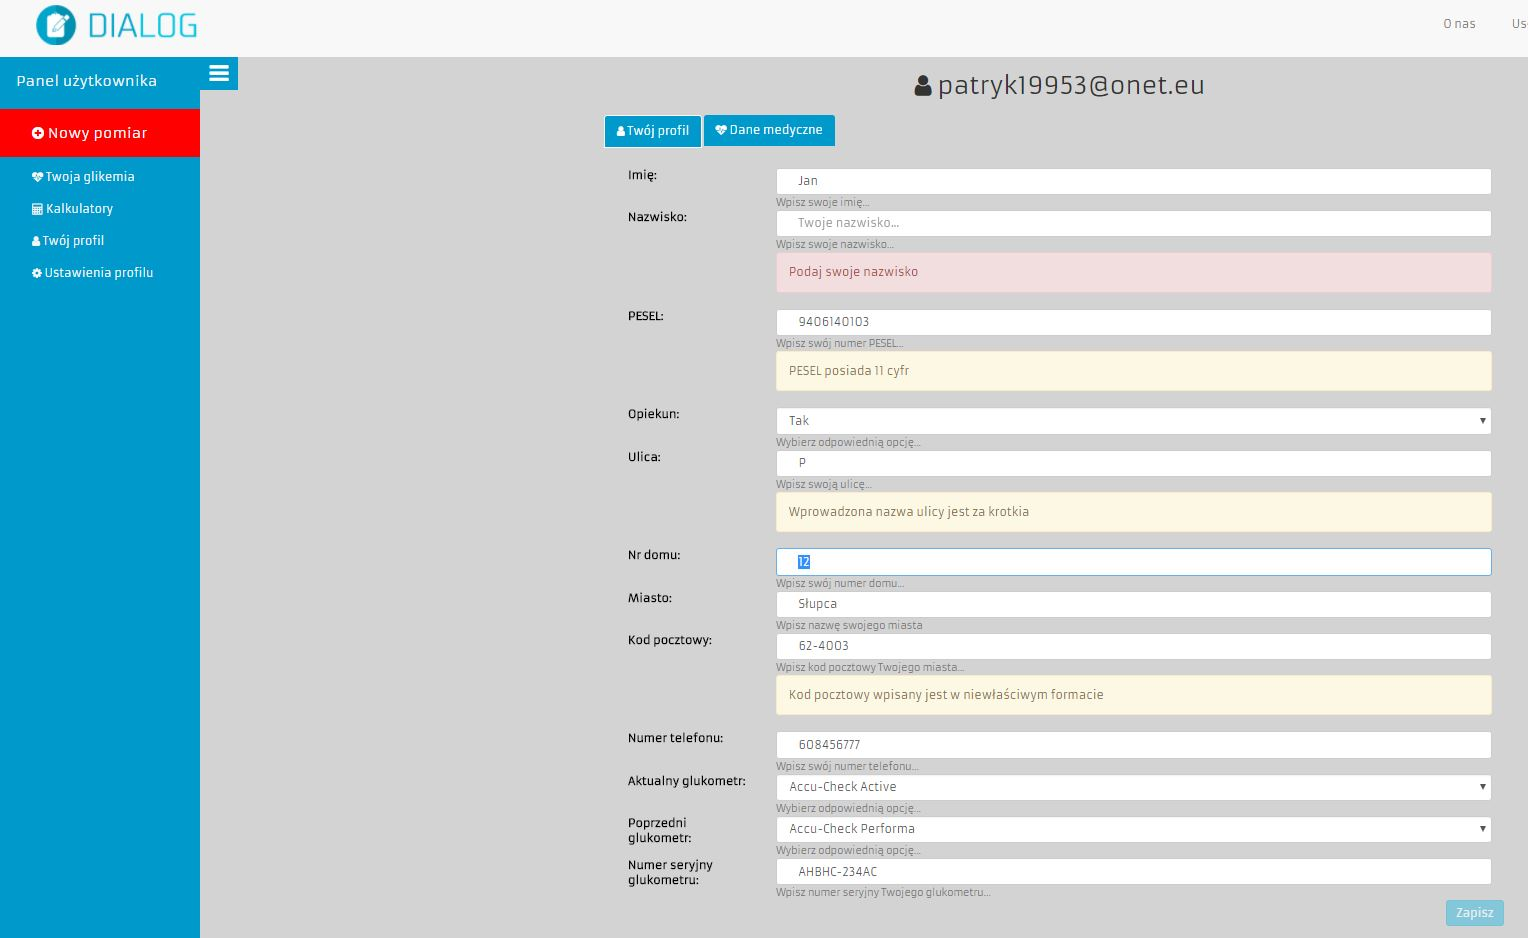
\includegraphics[scale=0.35]{images/form.JPG}
	\caption{Widok formularza z błędnie wypełnionymi polami i zablokowanym przyciskiem do zapisu ich wartości}
	\label{Rys:form}
\end{figure}



